%%%%%%%%%%%%%%%%%%%%%%%%%%%%%%%%%%%%%%
% LaTeX poster template
% Created by Nathaniel Johnston
% August 2009
% http://www.nathanieljohnston.com/2009/08/latex-poster-template/
%%%%%%%%%%%%%%%%%%%%%%%%%%%%%%%%%%%%%%

\documentclass[final]{beamer}
\usepackage[scale=1.4]{beamerposter}
\usepackage{graphicx}			% allows us to import images
\usepackage{algpseudocode}
\usepackage{algorithm}

%-----------------------------------------------------------
% Define the column width and poster size
% To set effective sepwid, onecolwid and twocolwid values, first choose how many columns you want and how much separation you want between columns
% The separation I chose is 0.024 and I want 4 columns
% Then set onecolwid to be (1-(4+1)*0.024)/4 = 0.22
% Set twocolwid to be 2*onecolwid + sepwid = 0.464
%-----------------------------------------------------------

\newlength{\sepwid}
\newlength{\introcolwid}
\newlength{\datacolwid}
\newlength{\threecolwid}
\setlength{\paperwidth}{48in}
\setlength{\paperheight}{36in}
\setlength{\sepwid}{0.024\paperwidth}
\setlength{\introcolwid}{0.22\paperwidth}
\setlength{\datacolwid}{0.34\paperwidth}
\setlength{\threecolwid}{0.708\paperwidth}
\setlength{\topmargin}{-0.5in}
\usetheme{confposter}
\usepackage{exscale}

\DeclareMathOperator*{\argmin}{arg\,min}

\newcommand{\red}[1]{{\color{red}#1}}
\newcommand{\green}[1]{{\color{green}#1}}
\newcommand{\blue}[1]{{\color{blue}#1}}

\newcommand{\Face}{\red{\textbf{Face}}}
\newcommand{\Place}{\green{\textbf{Place}}}
\newcommand{\Object}{\blue{\textbf{Object}}}
\newcommand{\Faces}{\red{\textbf{Faces}}}
\newcommand{\Places}{\green{\textbf{Places}}}
\newcommand{\Objects}{\blue{\textbf{Objects}}}

%-----------------------------------------------------------
% The next part fixes a problem with figure numbering. Thanks Nishan!
% When including a figure in your poster, be sure that the commands are typed in the following order:
% \begin{figure}
% \includegraphics[...]{...}
% \caption{...}
% \end{figure}
% That is, put the \caption after the \includegraphics
%-----------------------------------------------------------

\usecaptiontemplate{
\small
\structure{\insertcaptionname~\insertcaptionnumber:}
\insertcaption}

%-----------------------------------------------------------
% Define colours (see beamerthemeconfposter.sty to change these colour definitions)
%-----------------------------------------------------------

\setbeamercolor{block title}{fg=ngreen,bg=white}
\setbeamercolor{block body}{fg=black,bg=white}
\setbeamercolor{block alerted title}{fg=white,bg=dblue!70}
\setbeamercolor{block alerted body}{fg=black,bg=dblue!10}

%-----------------------------------------------------------
% Name and authors of poster/paper/research
%-----------------------------------------------------------

\title{Iterative LASSO: An even-handed approach to whole brain MVPA}
\author{Christopher Cox, Qihong Lu, Timothy Rogers}
\institute{University of Wisconsin--Madison}

%-----------------------------------------------------------
% Start the poster itself
%-----------------------------------------------------------

\begin{document}
\begin{frame}[t]
  \begin{columns}[t]												% the [t] option aligns the column's content at the top
    \begin{column}{\sepwid}\end{column}			% empty spacer column
    \begin{column}{\introcolwid}
      \begin{block}{Introduction}
      	\begin{itemize}
      		\item A large body of the most historically relevant work in cognitive neuroscience has emphasized \textbf{functional localization}. 
%      		\item There has been great emphasis on identifying brain regions that seem to be reliably and specifically active even for quite complex cognitive functions, such as face (ref), place (ref), and object (ref) recognition. 
      		\item However, the focus on \textit{reliability}, \textit{specificity}, and \textit{locality} of neural activity may reveal only a fraction of the full neural representation of these concepts and processes (ref), overlooking what is \textbf{distributed and idiosyncratic}.
      		\item We consider whether {\Face}, {\Place}, and {\Object} recognition are processes whose neural bases are specific, reliable, and localized systems, or if they have important aspects that are distributed and idiosyncratic.
      	\end{itemize}
      \end{block}
      \vskip2ex
      \begin{block}{Iterative Lasso}
      	Lasso (ref) is an example of regularized regression:
   		\begin{equation*}
			\argmin_\beta \sum^{n}_{i=1}{(\bar{y}_i - X_i\beta)^2} {\color{red} + \lambda h(\beta)}
%	   		\argmin_\beta \sum^{n}_{i=1}{\log(1 + e^{-\bar{y}_i X_i\beta})} {\color{red} + \lambda h(\beta)}
   		\end{equation*}

   		It is standard regression with an additional penalty:
		\begin{equation*}
	   		{\color{red}h(\beta)} = \sum|\beta_j|
   		\end{equation*}
   		Seeks best solution using {\em fewest} voxels. But that means many informative voxels may not be included in the solution. That is, \textbf{Lasso has a low hit-rate}.
   		
   		If Lasso is run \textbf{iteratively}, each time excluding voxels that have already been discovered, more of the activity contributing to neural state can be recovered. 

		 \begin{figure}
		 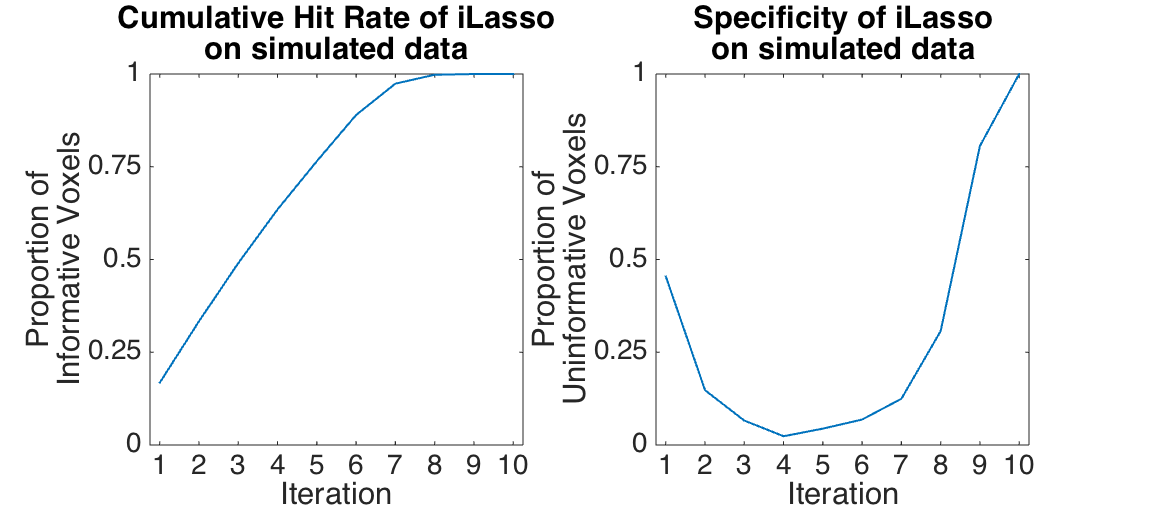
\includegraphics[width=\textwidth]{figures/HitRate_FalseAlarmRate.png}
		 \caption{Specificity of Iterative Lasso}
		 \end{figure}

      \end{block}
      \vskip2ex
      \begin{alertblock}{Lasso for fMRI analysis}
        Lasso achieves a sparse solution by selecting voxels that each provide \textit{unique} information. Is several voxels are very informative but are correlated, Lasso will select one and ignore the others. By running Lasso iteratively, these correlated voxels can be identified. 
      \end{alertblock}
    \end{column}
   	\begin{column}{\sepwid}\end{column}			% empty spacer column
   	\begin{column}{\introcolwid}
   		\begin{block}{Data}
   			\begin{itemize}
   				\item fMRI data from 10 Ps.
   				\item Ps viewed each of 30 celebritiy {\Faces}, 30 famous {\Places}, and 30 common {\Objects} in random order.
   				\item On each trial, the picture stayed on the screen for 5s. 
   				\item After it disappeared, Ps rated how much they liked the celebrity, how much they would like to visit the location, or how often they encountered the object in everyday life. 
   			\end{itemize}
   		\end{block}
   		
   		\begin{block}{Procedure}
				\begin{algorithmic}
					\ForAll {Subjects}
						X \gets SubjectData
						\ForAll {ROI \gets Face,Place,Object,WholeBrain}
							\For {TR \gets 0,4}
								solution \gets iLasso()				
							\EndFor
						\EndFor
					\EndFor
				\end{algorithmic}
  		\end{block}
  		\begin{block}{Performance}
			\begin{figure}
				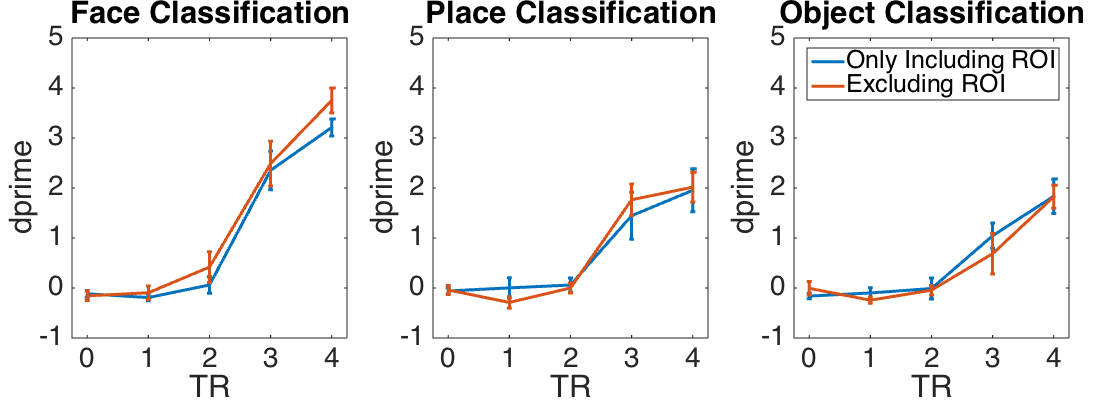
\includegraphics[width=\textwidth]{figures/Summary_by_TR.png}
				\caption{Classification performance, contrasting whether iLasso is trained on voxels only within, or only beyond, the prescribed ROIs. TR 0 is stimulus onset.}
			\end{figure}			
  		\end{block}
   	\end{column}

    \begin{column}{\sepwid}\end{column}			% empty spacer column
    \begin{column}{\introcolwid}					  % create a three-column-wide column and then we will split it up later
		\begin{block}{Data and ROIs}
			\begin{figure}
				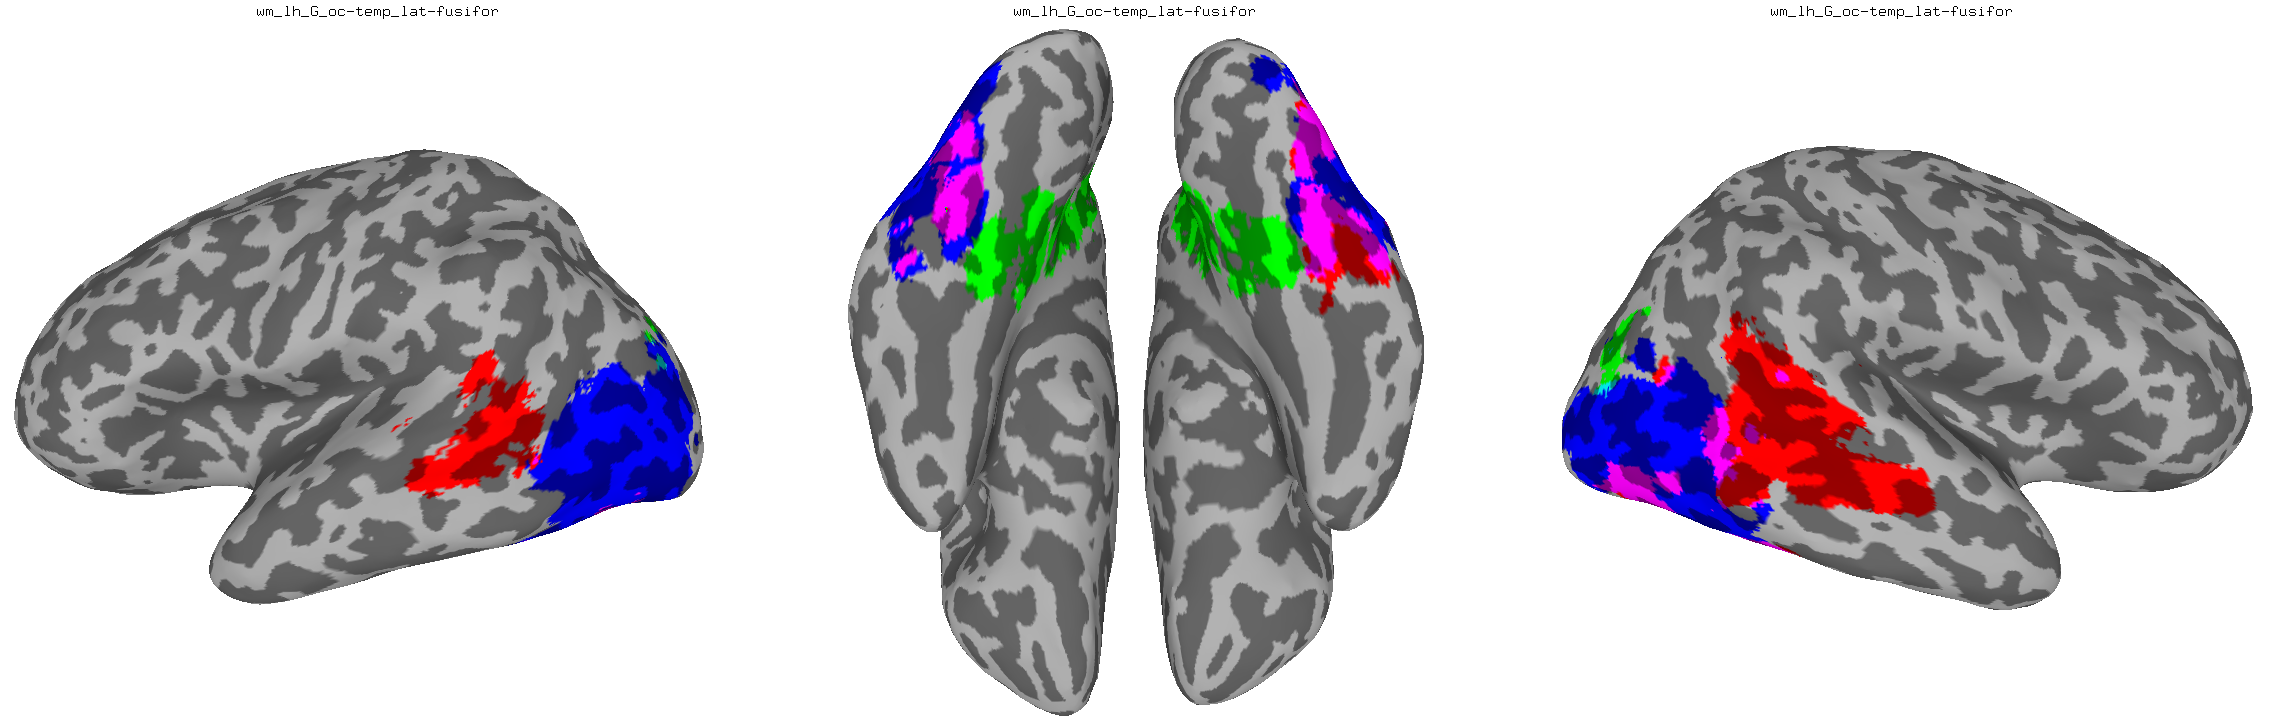
\includegraphics[width=\textwidth]{figures/ROIs.png}
				\caption{ROIs defined by Julian, J.B., Fedorenko, E., Webster, J., \& Kanwisher, N. (2012)}
			\end{figure}
		\end{block}
		
		\begin{block}{Whole-brain Solutions}
			\begin{figure}
				\includegraphics[width=\textwidth]{figures/face_gt5c_key.png}
				\caption{Face Solutions}
			\end{figure}
			\begin{figure}
				\includegraphics[width=\textwidth]{figures/place_gt5c_key.png}
				\caption{Place Solutions}
			\end{figure}
			\begin{figure}
				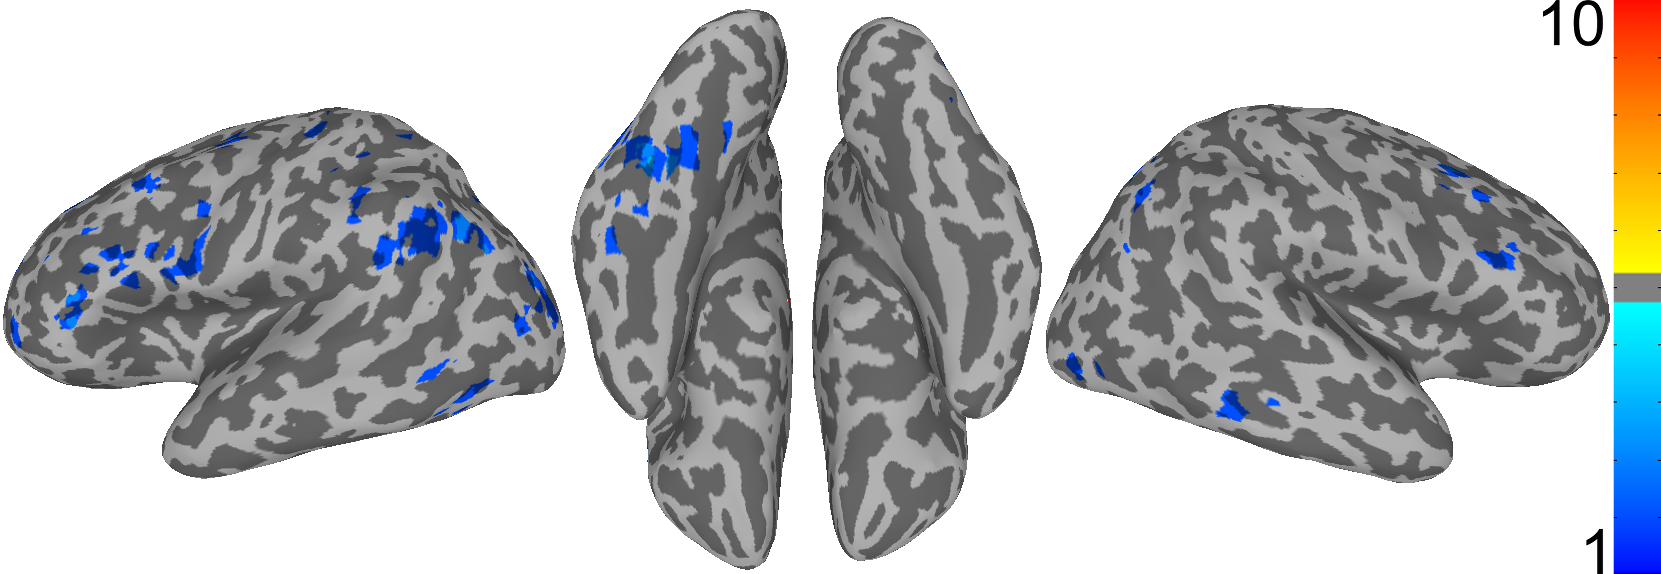
\includegraphics[width=\textwidth]{figures/object_gt5c_key.png}
				\caption{Object Solutions}
			\end{figure}
		\end{block}
%          \setbeamercolor{block title}{fg=red,bg=white}%frame color
%          \setbeamercolor{block body}{fg=black,bg=white}%body color
          \begin{block}{Aggregate}
			\begin{figure}
				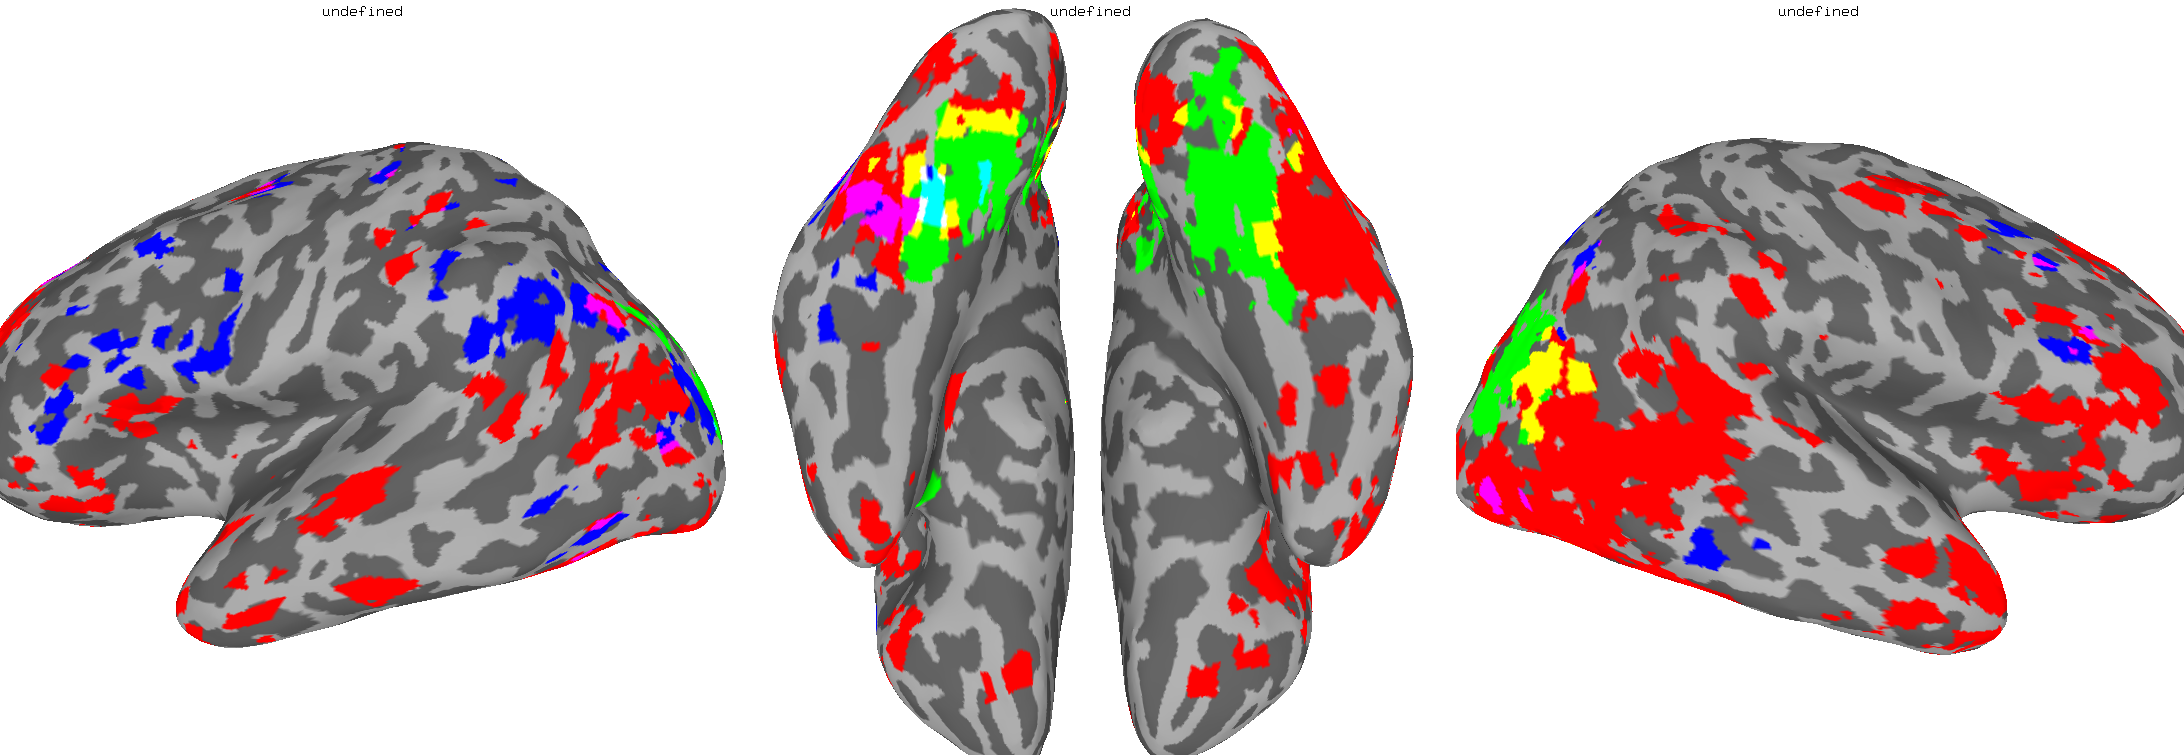
\includegraphics[width=\textwidth]{figures/FPO_gt5b2.png}
				\caption{Combined Solution Map}
			\end{figure}
          \end{block}
	\end{column}
	\begin{column}{\sepwid}\end{column}			% empty spacer column
	\begin{column}{\introcolwid}
      \setbeamercolor{block alerted title}{fg=black,bg=norange}	% frame color
      \setbeamercolor{block alerted body}{fg=black,bg=white}		% body color
      \begin{alertblock}{Alert Block Colours}
        You can similarly modify the colours for alert blocks (but try not to overdo it):\\
        \begin{semiverbatim}
          {\color{red}\\setbeamercolor}\{block title\}\newline \{fg=black,bg=norange\}
        \end{semiverbatim}
        \begin{semiverbatim}
          {\color{red}\\setbeamercolor}\{block  body\}\newline \{fg=black,bg=white\}
        \end{semiverbatim}
      \end{alertblock}        
    \end{column}
	\begin{column}{\sepwid}\end{column}			% empty spacer column
\end{columns}
\end{frame}
\end{document}
